\documentclass[margin=1pt]{standalone}

\usepackage{tikz}

\usetikzlibrary{
  calc,
  arrows, arrows.meta,
  decorations.pathreplacing,
  calligraphy,
}

\begin{document}
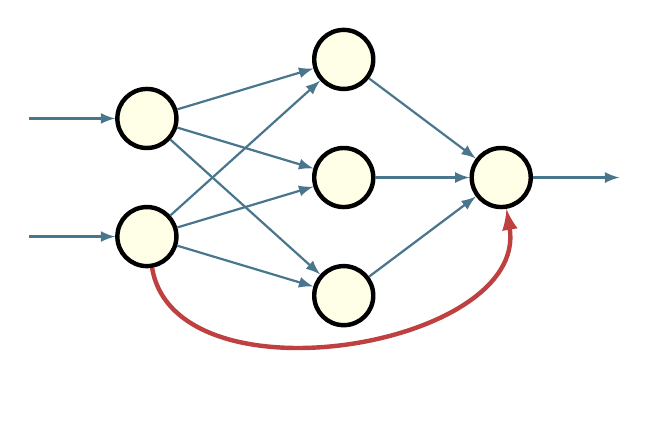
\begin{tikzpicture}[
    ultra thick,
    arr/.style={thick, cyan!50!black},
    lab/.style={font=\ttfamily, black},
    circ/.style={fill=yellow!10, draw=black, circle, minimum size=7.5mm},
  ]
  \node[circ] (w00) at (0,.75) {};
  \node[circ] (w01) at (0,-.75) {};

  \node[circ] (w10) at (2.5,1.5) {};
  \node[circ] (w11) at (2.5,0) {};
  \node[circ] (w12) at (2.5,-1.5) {};

  \node[circ] (w20) at (4.5,0) {};

  \foreach \j in {0,1,2} {
      \draw[arr, -latex] (w1\j) -- (w20);
      \foreach \i in {0,1} {
          \draw[arr, -latex] (w0\i) -- (w1\j);
        }
    }
  \foreach \i in {0,1} {
      \draw[arr, latex-] (w0\i) -- ++(-1.5,0);
    }
  \draw[arr, -latex] (w20) -- ++(1.5,0);

  \draw[arr, -latex, red!50!gray, ultra thick] (w01) to[bend right=90] (w20);

\end{tikzpicture}
\end{document}
